\documentclass[journal]{IEEEtran}
\usepackage{balance}
\usepackage{color}
\usepackage{float}
\usepackage{amssymb}
\usepackage{cite}
\usepackage{amsmath}
\usepackage{amsthm}
\newtheorem{Lemma}{Lemma}
\newtheorem{corollary}{Corollary}
\newtheorem{proposition}{Proposition}
\theoremstyle{remark}
\newtheorem{remark}{Remark}
\renewcommand\qedsymbol{}
\usepackage{enumerate}
\usepackage{algorithm}
\usepackage{algpseudocode}
\usepackage{graphicx}
\usepackage{epstopdf}
\epstopdfsetup{outdir=./}
\graphicspath{{images/}}
\usepackage{booktabs}
\usepackage{multirow}
\usepackage{bm}
\usepackage{url}
\usepackage{tabularx}
\usepackage{placeins}
% ---------------------------------------------------------------------------
% REVISION MARKUP.  \revision{} holds first-round changes and is now set plain,
% because that text is already part of the accepted record.  \revtwo{} holds
% second-round changes.  build_versions.py rewrites only the two lines below to
% produce the marked copy (\revtwo in red) and the clean copy (both plain).
% ---------------------------------------------------------------------------
\newcommand{\revision}[1]{#1}
\newcommand{\revtwo}[1]{\textcolor{blue}{#1}}
\newcommand{\revtwoeq}{\color{blue}}
\usepackage{etoolbox}
\AtBeginEnvironment{Lemma}{\color{black}}
\AtBeginEnvironment{corollary}{\color{black}}
\AtBeginEnvironment{proposition}{\color{black}}
\AtBeginEnvironment{proof}{\color{black}}
\AtBeginEnvironment{table}{\color{black}}
\AtBeginEnvironment{table*}{\color{black}}
\setlength{\textfloatsep}{4pt plus 1pt minus 1pt}
\setlength{\floatsep}{4pt plus 1pt minus 1pt}
\setlength{\intextsep}{4pt plus 1pt minus 1pt}
\setlength{\abovecaptionskip}{2pt plus 1pt minus 1pt}
\setlength{\belowcaptionskip}{1pt plus 1pt minus 1pt}
\setlength{\abovedisplayskip}{2pt plus 1pt minus 1pt}
\setlength{\belowdisplayskip}{2pt plus 1pt minus 1pt}
\setlength{\abovedisplayshortskip}{1pt plus 1pt minus 1pt}
\setlength{\belowdisplayshortskip}{1pt plus 1pt minus 1pt}
\setcounter{topnumber}{5}
\setcounter{bottomnumber}{5}
\setcounter{totalnumber}{10}
\renewcommand{\topfraction}{0.95}
\renewcommand{\bottomfraction}{0.90}
\renewcommand{\textfraction}{0.05}
\renewcommand{\floatpagefraction}{0.85}
\renewcommand{\dbltopfraction}{0.95}
\renewcommand{\dblfloatpagefraction}{0.85}

% Correct bad hyphenation here
\hyphenation{op-tical net-works semi-conduc-tor}

\begin{document}

\title{MAML-Select: An Online Adaptive Client Selection Method for Federated Learning via Meta-Learning}

%\author{Aakash Sharma, Advait Pathak, Ricktho Sarkar, Om Jee Pandey, \textit{Senior Member, IEEE}
%\thanks{A. Sharma, A. Pathak, and R. Sarkar are undergraduate researchers at IIT BHU Varanasi, Varanasi 221005, India.}
%\thanks{O. J. Pandey is with the Department of Electronics Engineering, IIT BHU Varanasi, Varanasi 221005, India (e-mail: omjee.ece@iitbhu.ac.in).}}

\maketitle

% =====================================================================
% ABSTRACT
% =====================================================================
\begin{abstract}
% \revision{Federated Learning (FL) enables collaborative model training across distributed edge data, however client selection remains difficult when devices differ in data distribution, compute capacity, energy state, and communication latency. Selecting only the fastest or most statistically useful clients can slow convergence, increase resource cost, or reduce participation coverage. System-aware selectors such as FedCS and TiFL address stragglers, while utility-aware methods such as Oort, FedCor, CriticalFL, and FedGCS use loss, correlation, critical-period, or generative signals to improve training. However, many existing methods rely on fixed scoring rules, costly modelling stages, or feedback that does not explicitly adapt the selector before every round. The remaining gap is a lightweight policy that can rapidly re-rank clients as their utility and system state change dynamically during FL. We propose \textbf{Model Agnostic Meta-Learning Select (MAML-Select)}, an online adaptive selector that treats each FL round as a meta-learning task. A compact Multilayer Perceptron (MLP) is adapted with a first order update of MAML-Select from recent local-loss and latency feedback, then used to score available clients before a query-set meta-update. Across Fashion-MNIST, CIFAR-10, and CIFAR-100 with $100$ clients, $K=10$, Dirichlet $\alpha=0.5$, and three seeds, MAML-Select reduces cumulative Tera Floating-Point Operations (TFLOPs) by up to $21.5\%$ and modelled energy by up to $24.7\%$ relative to FedAvg on all three datasets, with paired-test support ($p<0.05$). Accuracy remains competitive with FedAvg and FedGCS, with the largest trade-off on CIFAR-10. These findings suggest that meta-adaptive client selection can make edge AI deployments more resource-conscious.}
\revision{In Federated Learning (FL), choosing which clients update the shared model in each round is a combinatorial scheduling problem under resource constraints. Clients differ in data utility, training speed, battery capacity and bandwidth. Since only a small cohort can communicate per round, conventional client-selection strategies often favor clients with high training utility or fast updates, which repeatedly selects a narrow group of clients, leaves slower ones underused, and reduces participation coverage. Existing methods like FedCS and TiFL use system state to reduce straggler effects, whereas Oort, FedCor, CriticalFL, and FedGCS score clients using training utility, loss correlation, critical-period timing, or learned client combinations. However, these methods often rely on a fixed scoring rule, or update it slowly, even though a client’s usefulness changes as the global model evolves. \textbf{Model-Agnostic Meta-Learning Select (MAML-Select)} removes this fixed-rule assumption, and frames each round as a fast adaptation task. A lightweight policy network is learned using the previous round’s observed loss reduction and latency, and is used for ranking clients. % after one first-order MAML adaptation step using the previous round’s observed loss reduction and latency. 
After the selected clients return their updates, the same policy is meta-updated using the new feedback. We evaluate MAML-Select on Fashion-MNIST, CIFAR-10, and CIFAR-100 with 100 clients, K = 10 selected clients per round, a Dirichlet non-independent and identically distributed (non-IID) split with $\alpha=0.5$, and three random seeds. \revtwo{Against FedAvg on the three datasets in turn, MAML-Select lowers cumulative Tera Floating-Point Operations (TFLOPs) by $12.9\%$, $21.5\%$ and $1.7\%$ and modelled energy by $16.4\%$, $24.8\%$ and $4.7\%$, for accuracy changes of $-0.1$, $-3.8$ and $-1.5$ percentage points, and it lowers the mean CIFAR-100 round latency by $14.4\%$. The saving is small on CIFAR-100, where FedGCS is the stronger method on accuracy. Participation coverage stays at $100\%$ on every dataset by construction, through a single exploration slot.} %Overall, MAML-Select provides a resource-aware client-selection strategy with competitive accuracy and low client-training computational cost.
}
\end{abstract}
\renewcommand\IEEEkeywordsname{Impact Statement}
\begin{IEEEkeywords}
\revision{FL is central to privacy-preserving AI across heterogeneous environments, such as mobile health, intelligent transportation, and smart-city systems, but these face tight computational-capacity, energy-consumption, and latency budgets. MAML-Select contributes an adaptive selection mechanism that reduces client-training computational cost while preserving broad participation coverage. By using recent training feedback to re-rank clients, it supports FL systems that respond to changing device conditions instead of relying on a fixed rule. The reported energy values are modelled estimates that follow the declared simulator and device-tier setup, giving a transparent basis for comparing selection policies. The broader impact is a more resource-aware path for deploying distributed AI at the edge, including the industrial Internet of Things (IoT).}


%This enables more scalable and energy-efficient privacy-preserving AI on resource-constrained edge devices.
\end{IEEEkeywords}
\renewcommand\IEEEkeywordsname{Index Terms}
\begin{IEEEkeywords}
Federated learning, client selection, meta-learning, computational efficiency.
\end{IEEEkeywords}
% =====================================================================
% I. INTRODUCTION
% =====================================================================
\section{Introduction}

\IEEEPARstart{F}{ederated} Learning (FL) trains a shared model across many devices without moving their raw data to the server~\cite{mcmahan2017communication}. \revision{Clients train locally and share only model updates, but differ in hardware, network conditions, and data. This creates drift under non-independent and identically distributed (non-IID) data and straggler delays in synchronous training}~\cite{karimireddy2020scaffold,mai2024study,tapwal2026stragglers,forootani2026asynchronous,borazjani2026redefining}. The problem of \textit{whom to select} each round remains open.

Client selection chooses a subset $\revision{\mathcal{S}_t} \subset \{1, \ldots, N\}$ each round. \revision{Client utility is non-stationary, because a useful client can become redundant later, while an overlooked client can become important in the long run.} System-aware methods improve participation but can leave slow yet data-rich clients underused~\cite{nishio2019client,chai2020tifl}, and utility-aware methods prioritize information gain at the cost of latency or expensive server-side modelling~\cite{lai2021oort,tang2022fedcor,xu2024federated,yan2023criticalfl,ning2024fedgcs}. Learning-based selectors use histories, features, or reinforcement signals~\cite{wang2020optimizing,pan2024contextual,kazemi2026robust}. \revision{A round-by-round mechanism for adapting the policy to evolving utility remains underexplored.}

\revision{We propose MAML-Select, a client-selection framework based on a Model-Agnostic Meta-Learning (MAML)-style fast adaptation step~\cite{finn2017model}, which learns the policy network via recent feedback before the next ranking decision. Unlike reinforcement-learning (RL)-based or contextual-bandit selectors, the proposed MAML-Select uses rapid gradient-based policy adaptation. Unlike personalization of FL client models}~\cite{fallah2020personalized}, \revision{the proposed MAML adapts the selector, rather than the client model. The approach suits devices with limited computational capacity, strict deadlines, or intermittent connectivity.} The contributions are as follows.
\begin{enumerate}
\setlength{\itemsep}{0pt}
\setlength{\topsep}{1pt}
		\item We formulate the FL client selection problem as a meta-learning task and introduce the MAML-Select algorithm with \revision{rapid gradient-based} adaptation for online client selection.
        \item \revision{Experiments on Fashion-MNIST, CIFAR-10, and CIFAR-100 under non-IID settings ($\alpha = 0.5$, three seeds) show that MAML-Select delivers accuracy competitive with FedAvg and FedGCS at lower computational cost, and higher accuracy than FedCS, Oort, TiFL, and FedCor. Sensitivity and ablation studies over $\lambda$, the inner-loop steps, the selector width, and the state features support the design choices.}
		\item We demonstrate that MAML-Select \revision{\textit{lowers cumulative training TFLOPs} by up to $21.5\%$ and modelled energy consumption by up to $24.7\%$ relative to FedAvg, with paired-test support for the resource reductions}.
\end{enumerate}

\textit{Organization.} The rest of this paper is organized as follows. Section~II reviews related work on client selection in FL. Section~III details the system model and problem formulation. The proposed MAML-Select algorithm is described in Section~IV, followed by evaluation and results in Section~V. Section~VI concludes this paper and discusses future research directions.

% =====================================================================
% II. RELATED WORK
% =====================================================================
\section{Related Work}
\subsection{System-Aware Selection}
System-aware selection addresses stragglers. FedCS selects feasible clients under resource constraints, while TiFL groups devices into online performance tiers~\cite{nishio2019client,chai2020tifl}. Recent studies show similar concerns for slow but data rich clients in resource-constrained medical IoT and asynchronous FL with heterogeneous objectives~\cite{tapwal2026stragglers,forootani2026asynchronous}. MAML-Select uses feedback from the previous training phase, and learns the selection policy from six client-state features. %while learning how much they should matter in the current training phase.

\subsection{Data-Aware and Utility-Based Selection}
Data-aware methods select clients for model utility rather than speed alone. Oort prioritizes data-rich and fast clients, and FedCor models correlations between client losses~\cite{lai2021oort,tang2022fedcor}. CriticalFL uses critical learning periods, while FedGCS searches for client combinations in a learned continuous space~\cite{yan2023criticalfl,ning2024fedgcs}. Other work couples selection with aggregation design~\cite{xu2024federated,tran2026fedimp}. MAML-Select instead targets rapid adaptation of the ranking policy as client utility evolves.

\subsection{Learning-Based and Meta-Learning Approaches}
Learning-based selectors improve from observed feedback. FAVOR uses a deep Q-network, while neural contextual bandits learn from client features and rewards~\cite{wang2020optimizing,pan2024contextual}, and recent work studies deep-RL selection for robustness and fairness-aware participation~\cite{kazemi2026robust,arisdakessian2026vox}. MAML is used in~\cite{fallah2020personalized} to personalize client models, whereas MAML-Select adapts the server-side ranking policy instead.

\revision{Table~\ref{tab:related_work_comparison} consolidates these distinctions. For methods without a stated closed-form selection complexity, it reports the dominant server-side operation.}

\begin{table*}[!t]
    \color{black}
    \caption{Comparison of representative methods and MAML-Select.}
    \label{tab:related_work_comparison}
    \centering
    \scriptsize
    \setlength{\tabcolsep}{3pt}
    \renewcommand{\arraystretch}{0.98}
    \begin{tabularx}{\textwidth}{lXXX}
        \toprule
        \textbf{Method} & \textbf{Primary objective} & \textbf{Adaptation mechanism} & \textbf{Selection complexity or dominant operation} \\
        \midrule
        FedCS~\cite{nishio2019client} & Increase feasible updates under resource constraints & Resource estimates before selection & Resource-constrained subset search \\
        TiFL~\cite{chai2020tifl} & Mitigate stragglers while preserving accuracy & Online tier updates & Tiering and probabilistic sampling \\
        Oort~\cite{lai2021oort} & Improve time-to-accuracy & Utility and speed feedback & Utility scoring and guided sampling \\
        FedCor~\cite{tang2022fedcor} & Accelerate convergence under non-IID data & Loss-correlation model & Gaussian process (GP) covariance operations \\
        FAVOR~\cite{wang2020optimizing} & Counterbalance non-IID bias & Experience-driven policy updates & DQN inference and training \\
        NCCB~\cite{pan2024contextual} & Learn contextual client combinations & Client features and reward feedback & Locality-sensitive hashing (LSH) feature extraction and bandit updates \\
        FedCG~\cite{xu2024federated} & Couple selection and gradient compression & Capability-aware compression updates & Submodular optimization and linear programming \\
        CriticalFL~\cite{yan2023criticalfl} & Exploit critical learning periods & Period-aware participation & Base-selector dependent \\
        FedGCS~\cite{ning2024fedgcs} & Optimize client combinations & Search in a learned continuous space & Latent-space optimization and beam search \\
        Kazemi et al.~\cite{kazemi2026robust} & Improve robustness under poisoning attacks & Experience-driven policy updates & Deep-RL inference and training \\
        Vox Populi~\cite{arisdakessian2026vox} & Promote fair and inclusive participation & Fairness-aware client selection & Framework-dependent \\
        Per-FedAvg~\cite{fallah2020personalized} & Personalize the client model to local data & MAML adapts the client model, not the selector & No client selection, only per-client fine-tuning \\
        \textbf{MAML-Select} & Adapt rankings under evolving client utility & Fast adaptation from recent round feedback & $\mathcal{O}(N|\phi|)$ scoring plus a gradient-adaptation step \\
        \bottomrule
    \end{tabularx}
\end{table*}

\revision{\textbf{Difference from prior work.} MAML-Select meta-learns the selection policy $h_\phi$. Unlike heuristic, RL, contextual-bandit, and generative selectors, it uses a MAML inner update to convert recent feedback into fast policy weights before the next cohort is scored. A fixed heuristic or bandit may update rewards over time, but does not adapt the scoring-network parameters from a support set immediately before selection.}

% =====================================================================
% III. SYSTEM MODEL AND PROBLEM FORMULATION
% =====================================================================
\section{System Model and Problem Formulation}

\begin{figure}[!t]
\centering
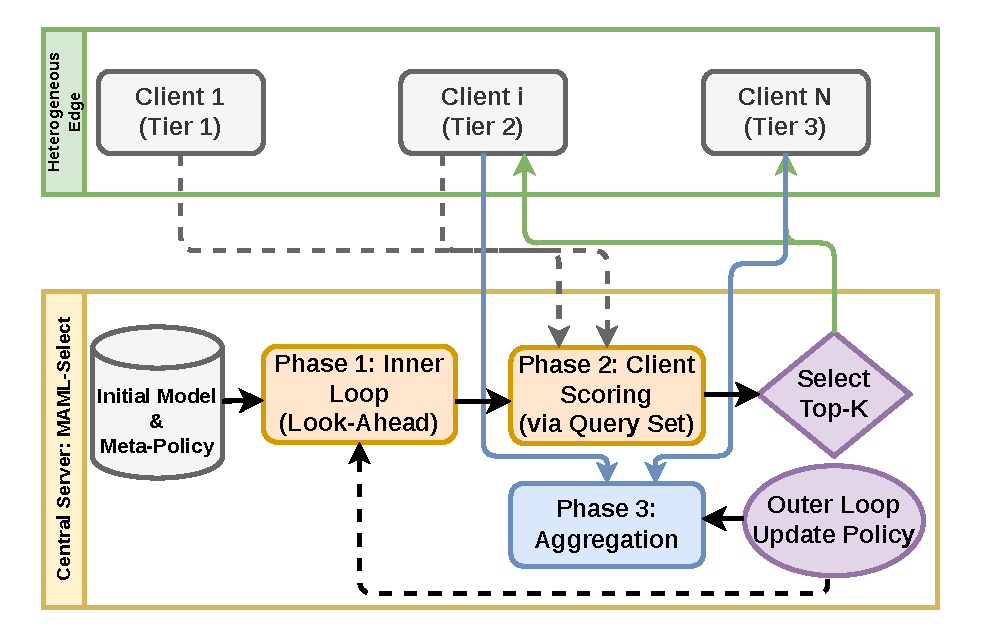
\includegraphics[width=0.86\columnwidth]{MAML.pdf}
\caption{\revtwo{System model and the per-round workflow of MAML-Select. The server holds the global model and the ranking policy $h_\phi$. At the start of round $t$ it adapts the policy on the support set and meta-updates it on the query set, both drawn from completed rounds, then scores the available clients and broadcasts to the selected cohort $\mathcal{S}_t$. The cohort trains locally and returns updates with the loss and resource feedback that forms the next round's sets.}}
\label{fig:system_model}
\end{figure}

\revision{We consider a central server and $N$ heterogeneous clients indexed by $\mathcal{N} = \{1, 2, \ldots, N\}$. Client $i$ stores a local dataset $\mathcal{D}_i$ with $n_i$ samples.} The global objective is to minimize the empirical risk over the distributed data as
\begin{equation}
	\min_{\theta \in \mathbb{R}^d} F(\theta) = \sum_{i=1}^{N} \frac{n_i}{n} F_i(\theta),
	\label{eq:global_objective}
\end{equation}
\revision{where $\theta \in \mathbb{R}^d$ denotes the global model, $n = \sum_{i=1}^{N} n_i$, and $F_i(\theta) = \frac{1}{n_i} \sum_{j=1}^{n_i} \ell(\theta; x_{i,j}, y_{i,j})$ is the local empirical risk, with $\ell(\cdot)$ the per-sample loss (e.g.\ cross-entropy).}

\revision{Fig.~\ref{fig:system_model} shows the setting and the order of operations in one round. At round $t$, let $\mathcal{A}_t \subseteq \mathcal{N}$ be the available clients and $\mathcal{S}_t \subseteq \mathcal{A}_t$ the selected cohort. The server holds the global model and the policy, while clients keep data local and return only updates, loss summaries, and resource-state feedback, so selection is a server-side decision taken before each broadcast.}

\revision{Client $i$ has per-round latency $T_{i,t}=T_{i,t}^{comp}+T_{i,t}^{comm}$.} \revtwo{The computation time is $T_{i,t}^{comp}=E\,n_i/f_{i,t}$ over $E$ local epochs and $n_i$ samples, where $f_{i,t}$ is the device throughput in samples per second, set by its hardware tier. The per-sample model cost is absorbed into it. The communication time is $T_{i,t}^{comm}=n_i/(\kappa B_{i,t})$ for a payload scale $\kappa$ and uplink quality $B_{i,t}$}~\cite{nishio2019client}\revtwo{, and it stays under $1\%$ of $T_{i,t}^{comp}$ here, so local training dominates.} \revision{In synchronous FL the slowest selected client sets the latency,}
\begin{equation}
	\color{black}
	T_t^{round} = \max_{i \in \mathcal{S}_t} T_{i,t}.
	\label{eq:round_latency}
\end{equation}


\revision{Let $a_{i,t}$ indicate whether client $i$ is selected. Under policy $\pi_\phi$, the constrained client-selection problem is}
\begin{equation}
	\color{black}
	\begin{aligned}
		\min_{\pi_\phi}\quad & \sum_{t=1}^{T} \left[F(\theta_{t+1}) + \lambda T_t^{round}\right] \\
		\text{s.t.}\quad & \sum_{i=1}^{N} a_{i,t}=K,\quad a_{i,t}\in\{0,1\}, \\
		& a_{i,t}\leq \mathbf{1}\{i\in\mathcal{A}_t\},		
	\end{aligned}
	\label{eq:bi_objective}
\end{equation}
\revision{where $K$ is the cohort size, $T$ is the number of rounds, and $\lambda \geq 0$ controls the trade-off between latency and loss, and the client selection subset is updated as $\mathcal{S}_t=\{i:a_{i,t}=1\}$. A larger $\lambda$ places more emphasis on latency, while $\lambda=0$ yields loss-only selection. We assume $|\mathcal{A}_t|\geq K$. The model $\theta_{t+1}$ results from local training and aggregation over $\mathcal{S}_t$. The problem remains challenging because the action space is combinatorial and client utility evolves during training.}

% =====================================================================
% IV. METHODOLOGY: MAML-SELECT
% =====================================================================
\section{MAML-Select Algorithm}
\revision{Building on~\eqref{eq:bi_objective}, MAML-Select treats selection as a meta-learning problem, since client utility changes during training.}

\subsection{State Space}
\revision{The server builds a state vector $\bm{s}_{i,t} \in \mathbb{R}^6$ for each client $i$ at round $t$. It holds the local training loss $\hat{L}_{i,t}$, the gradient norm $\|\nabla F_i\|_2$, the estimated latency $\hat{T}_{i,t}$, the battery level $b_{i,t}$, the selection frequency $\nu_{i,t}$, and the staleness $\tau_{i,t}$ measured in rounds since the client was last selected}~\cite{pan2024contextual,xu2024federated}. The three pairs capture statistical utility, system feasibility, and participation balance. Each round $t$ is a task $\mathcal{T}_t$ in which clients are ranked so the top-$K$ cohort minimizes the per-round cost.

\revtwo{The six raw entries carry different physical units. Before they reach the policy, each column is therefore standardized across the clients available in that round,}
\begin{equation}
	\revtwoeq
	\bm{s}_{i,t} \leftarrow \bigl(\bm{s}^{raw}_{i,t}-\bm{\mu}_t\bigr)\oslash\bigl(\bm{\sigma}_t+\epsilon_0\bigr),
	\label{eq:zscore}
\end{equation}
\revtwo{where $\bm{\mu}_t,\bm{\sigma}_t$ are the per-feature mean and standard deviation over $\mathcal{A}_t$, $\oslash$ is elementwise division, and $\epsilon_0=10^{-8}$. The policy input is then dimensionless and the score is a relative ranking within one round, which is all Top-$K$ needs.}

MAML-Select trains a meta-policy network $h_\phi(\bm{s}_{i,t})$, parameterized by $\phi$, which is adapted to the current round using recent feedback. \revision{The policy is a $6$-$64$-$64$-$1$ multilayer perceptron (MLP) with rectified linear unit (ReLU) activations and 4,673 trainable parameters.} \revtwo{Cost feedback for a cohort becomes observable only after that cohort has finished training, so the two meta-learning sets are drawn from two consecutive completed rounds. Writing $\mathcal{S}_t$ for the cohort of round $t$, the support and query sets used at round $t$ are}
\begin{equation}
	\revtwoeq
	\begin{aligned}
	\mathcal{D}_{sup}(t) &= \bigl\{(\bm{s}_{i,t-2},c_{i,t-2})\bigr\}_{i\in\mathcal{S}_{t-2}}, \\
	\mathcal{D}_{query}(t) &= \bigl\{(\bm{s}_{i,t-1},c_{i,t-1})\bigr\}_{i\in\mathcal{S}_{t-1}} ,
	\end{aligned}
	\label{eq:sets}
\end{equation}
\revtwo{and therefore $\mathcal{D}_{sup}(t)=\mathcal{D}_{query}(t-1)$. This lag is what makes the procedure a meta-learning problem rather than online regression, because the inner step adapts on an older round while the meta-gradient is measured on a newer one. The outer update therefore rewards initializations from which one adaptation step transfers forward in time, which is what a selector needs when utility drifts. The candidate set $\mathcal{D}_{cand}(t)=\{\bm{s}_{i,t}\mid i\in\mathcal{A}_t\}$ carries no labels and is only scored.}

\subsection{\revtwo{From the Cohort Objective to a Per-Client Score}}
\revtwo{The objective in~\eqref{eq:bi_objective} is defined over cohorts, whereas the selector ranks clients individually. We connect the two in two steps, and only the second is inexact.}

\revtwo{First, the straggler term is a maximum and is therefore not separable. For any deadline $T_{target}>0$ and any cohort $\mathcal{S}_t$,}
\begin{equation}
	\revtwoeq \frac{T_t^{round}}{T_{target}}\;\le\;1+\sum_{i\in\mathcal{S}_t}\rho_{i,t},\qquad
	\rho_{i,t}\,=\,\frac{\bigl(T_{i,t}-T_{target}\bigr)_{+}}{T_{target}},
	\label{eq:straggler_bound}
\end{equation}
\revtwo{where $(x)_+=\max(0,x)$. The left side is at most $1$ when every selected client meets the deadline, and otherwise the slowest client $j$ contributes $1+\rho_{j,t}\le 1+\sum_i\rho_{i,t}$. The bound never understates the latency cost, makes it additive, and renders the penalty dimensionless so it can be traded against a loss reduction through one unitless weight $\lambda$.}

\revtwo{Second, the risk decrease $F(\theta_t)-F(\theta_{t+1})$ is unknown when the cohort is chosen, so we replace it by $\sum_{i\in\mathcal{S}_t}\Delta_{i,t}$, the observable local loss reductions $\Delta_{i,t}=\hat{L}^{before}_{i,t}-\hat{L}^{after}_{i,t}$ over the $E$ local epochs. This is the one approximation in the derivation. It treats cohort contributions as additive and equates local with global progress, ignoring client drift and interference between updates, and we adopt it because it needs no validation set and no extra communication.}

\revtwo{Substituting~\eqref{eq:straggler_bound} and this surrogate into the per-round term of~\eqref{eq:bi_objective} and dropping the additive constant $\lambda$ gives a cohort surrogate that is modular in $\mathcal{S}_t$,}
\begin{equation}
	\revtwoeq \widetilde{F}_t(\mathcal{S})=\sum_{i\in\mathcal{S}}c_{i,t},\qquad
	c_{i,t}=\lambda\,\rho_{i,t}\;-\;\Delta_{i,t} ,
	\label{eq:cost}
\end{equation}
\revtwo{which is the per-client cost used throughout this work and the quantity the policy is trained to predict. Both terms are dimensionless, since $\rho_{i,t}$ is a fractional deadline overrun and $\Delta_{i,t}$ a loss difference. The deadline $T_{target}$ is the mean expected round latency of the Tier-2 devices, recomputed every round, with the pool median used if none is available.}

\begin{proposition}[\revtwo{Top-$K$ is exact for the surrogate}]\label{prop:topk}
\revtwo{Let $\mathcal{S}^\star$ hold $K$ indices of $\mathcal{A}_t$ with the smallest $c_{i,t}$. Then $\mathcal{S}^\star$ minimizes $\widetilde{F}_t$ over all subsets of $\mathcal{A}_t$ of size $K$.}
\end{proposition}
\begin{proof}
\revtwo{Suppose some feasible $\mathcal{S}$ has a smaller objective. Since both sets have size $K$, there are $u\in\mathcal{S}\setminus\mathcal{S}^\star$ and $v\in\mathcal{S}^\star\setminus\mathcal{S}$ with $c_{v,t}\le c_{u,t}$. Swapping $u$ for $v$ does not increase the objective and strictly reduces $|\mathcal{S}\setminus\mathcal{S}^\star|$, so at most $K$ swaps turn $\mathcal{S}$ into $\mathcal{S}^\star$ without ever increasing it, a contradiction.}
\end{proof}

\revtwo{The chain is therefore an exact bound, one stated approximation, and an exact combinatorial step. One gap remains, since $c_{i,t}$ depends on quantities realized only after client $i$ has trained, and the meta-policy fills it by predicting $c_{i,t}$, after which Proposition~\ref{prop:topk} applies to the predicted costs. The cohort therefore exactly optimizes a stated modular surrogate under predicted costs.}

\subsection{The MAML-Select Algorithm}\label{sec:method_selection}
The algorithm proceeds in three phases per round\revtwo{, all executed at the start of round $t$ in the order below. Both meta-learning updates therefore complete before any client is scored, and they use only the lagged feedback of~\eqref{eq:sets}, so no quantity from round $t$ selects the cohort of round $t$}.

\textbf{Phase~1, inner loop adaptation.}
\revision{At the start of round $t$ the server adapts $\phi_t$ on $\mathcal{D}_{sup}(t)$ with one gradient step,}
\begin{equation}
	\color{black}
		\phi'_t = \phi_t - \beta \nabla_{\phi_t} \mathcal{L}_{sup}(h_{\phi_t};\mathcal{D}_{sup}(t)),
		\label{eq:inner_loop}
\end{equation}
where $\mathcal{L}_{sup}$ is the mean-squared-error (MSE) loss between predicted scores and observed costs \revtwo{from round $t-2$}, and $\beta$ is the inner learning rate\revtwo{. The step is plain gradient descent with $\beta=0.01$ and a single inner step}.

{\color{black}
\begin{Lemma}[Inner-step descent]\label{stmt:inner}
Let the support loss $g_t(\phi)=\mathcal{L}_{sup}(h_\phi;\mathcal{D}_{sup}(t))$ be $L$-smooth, that is, $\nabla g_t$ is $L$-Lipschitz. If the inner step size obeys $0<\beta<2/L$, the inner update~\eqref{eq:inner_loop} is a descent step on the support loss,
\[
g_t(\phi'_t)\le g_t(\phi_t)-\beta\Bigl(1-\tfrac{L\beta}{2}\Bigr)\lVert\nabla g_t(\phi_t)\rVert_2^2 .
\]
\end{Lemma}
\begin{proof}
By $L$-smoothness, $g_t$ obeys the descent lemma
\[
g_t(\psi)\le g_t(\phi)+\nabla g_t(\phi)^{\top}(\psi-\phi)+\tfrac{L}{2}\lVert\psi-\phi\rVert_2^2 .
\]
Substituting $\psi=\phi'_t$, $\phi=\phi_t$, and the inner update $\phi'_t-\phi_t=-\beta\nabla g_t(\phi_t)$ yields the stated bound. Its coefficient $\beta(1-L\beta/2)$ is positive precisely for $0<\beta<2/L$, so the step never increases $g_t$ and strictly decreases it unless $\nabla g_t(\phi_t)=0$.
\end{proof}
A single support-set step therefore reduces the ranking loss, which justifies adapting before the candidates are scored.
}

\textbf{Phase~2\revtwo{, outer loop meta-update}.}
\revision{%The selected clients perform standard FL training.
The meta-policy is updated on \revtwo{the query set of~\eqref{eq:sets}},}
\begin{equation}
		\color{black}
		\phi_{t+1} \leftarrow \phi_t - \eta \nabla_{\phi'_t} \mathcal{L}_{query}(h_{\phi'_t}; \mathcal{D}_{query}(t)),
		\label{eq:outer_loop}
\end{equation}
\revision{where $\eta$ is the meta-learning rate. %We use a first-order MAML-style approximation: the
Query-loss gradient is evaluated at the adapted weights $\phi'_t$ and applied to the meta-parameters $\phi_t$, which omits the second-order derivatives.} \revtwo{Because $\mathcal{D}_{query}(t)$ is the feedback of round $t-1$ and $\mathcal{D}_{sup}(t)$ that of round $t-2$, this update measures how well one adaptation step on older feedback predicts the round that followed it. In the implementation the direction $\nabla_{\phi'_t}\mathcal{L}_{query}$ is applied through Adam at $\eta=10^{-3}$ rather than by plain descent, and Remark~\ref{rem:reading} states what this means for the analysis.}

\textbf{Phase~3\revtwo{, selection and FL execution}.}
\revision{The adapted $h_{\phi'_t}$ scores $\mathcal{A}_t$ and takes the $K$ lowest predicted costs,}
\begin{equation}
	\color{black}
	\mathcal{S}_t = \operatorname{Top-}K_{i \in \mathcal{A}_t} \left( -h_{\phi'_t}(\bm{s}_{i,t}) \right).
	\label{eq:selection}
\end{equation}
\revtwo{Two rules qualify~\eqref{eq:selection}. During the first $\lceil N/K\rceil$ rounds the policy has too little feedback to rank anything, so a cold start takes the cohort in a fixed seed-shuffled coverage order that visits every client once. Thereafter an exploration slot gives one of the $K$ places to the available client of largest staleness $\tau_{i,t}$, ties broken by the smallest selection frequency $\nu_{i,t}$ and then by the coverage order, and the rest to the Top-$(K-1)$ of the learned ranking. The slot is deterministic, is set to $\varepsilon=1$, and bounds how long any client can stay unobserved. Sec.~\ref{sec:fairness_recheck} verifies that coverage does not depend on the cold start.}

\revision{The selected clients then train, and their states and realized costs become the query set of round $t+1$ and the support set of round $t+2$. Algorithm~\ref{alg:maml_select} gives the full procedure.}

{\color{black}
\begin{Lemma}[Outer-step descent]\label{stmt:outer}
Let the query loss $q_t(\phi)=\mathcal{L}_{query}(h_\phi;\mathcal{D}_{query}(t))$ be $L_q$-smooth, and let
\[
\delta_t\,=\,\lVert\nabla q_t(\phi'_t)-\nabla q_t(\phi_t)\rVert_2
\]
denote the \revtwo{\emph{look-ahead displacement}}, the gap between the direction actually applied, $\nabla q_t(\phi'_t)$ at the adapted weights, and the query gradient $\nabla q_t(\phi_t)$ at the un-adapted weights. If $0<\eta\le 1/L_q$, the meta-update~\eqref{eq:outer_loop} satisfies
\[
q_t(\phi_{t+1})\le q_t(\phi_t)-\tfrac{\eta}{2}\lVert\nabla q_t(\phi_t)\rVert_2^2+\tfrac{\eta}{2}\delta_t^2 ,
\]
with the inner step controlling it through $\delta_t\le L_q\beta\lVert\nabla g_t(\phi_t)\rVert_2$.
\end{Lemma}
\begin{proof}
Write $\phi_{t+1}=\phi_t-\eta\,d_t$ with $d_t:=\nabla q_t(\phi'_t)$. With $\eta\le 1/L_q$, the descent lemma for $q_t$ gives
\[
q_t(\phi_{t+1})\le q_t(\phi_t)-\eta\,\nabla q_t(\phi_t)^{\top}d_t+\tfrac{\eta}{2}\lVert d_t\rVert_2^2 .
\]
Completing the square with $-a^{\top}b+\tfrac12\lVert b\rVert_2^2=\tfrac12\lVert b-a\rVert_2^2-\tfrac12\lVert a\rVert_2^2$, for $a=\nabla q_t(\phi_t)$ and $b=d_t$, gives
\[
q_t(\phi_t)-\tfrac{\eta}{2}\lVert\nabla q_t(\phi_t)\rVert_2^2+\tfrac{\eta}{2}\lVert d_t-\nabla q_t(\phi_t)\rVert_2^2 .
\]
Since $\lVert d_t-\nabla q_t(\phi_t)\rVert_2=\delta_t$, the first bound follows. The second uses $L_q$-smoothness and~\eqref{eq:inner_loop}, which give $\delta_t\le L_q\lVert\phi'_t-\phi_t\rVert_2=L_q\beta\lVert\nabla g_t(\phi_t)\rVert_2$.
\end{proof}
Since the bound makes $\delta_t$ proportional to $\beta$ for a bounded support-gradient norm, the error term $\tfrac{\eta}{2}\delta_t^2=\mathcal{O}(\beta^2)$ is \revtwo{small} at $\beta=10^{-2}$, and the first-order meta-update behaves like \revtwo{gradient descent on the query loss up to that $\mathcal{O}(\beta^2)$ floor}.

\revtwo{Two clarifications follow. First, $\delta_t$ measures how far the applied direction sits from the query gradient at $\phi_t$, which is what the descent inequality needs, and Lemma~\ref{stmt:outer} controls that displacement. Second, a rate follows only if the query objective is fixed across rounds, which is untenable here. Since $\mathcal{D}_{sup}(t)=\mathcal{D}_{query}(t-1)$, setting $q_t\equiv q$ would force $g_t\equiv q$ and collapse the problem into descent on a fixed loss, and it would assert that client utility never changes, which Sec.~\ref{sec:selector_convergence} shows is false. We therefore state a tracking bound.}

\begin{corollary}[\revtwo{Tracking under a drifting query objective}]\label{cor:rate}
\revtwo{Let Lemma~\ref{stmt:outer} hold at every round with $0<\eta\le 1/L_q$, let $q_t\ge q_{\min}$ for every $t$, and let $V_T=\sum_{t=1}^{T}(q_{t+1}(\phi_{t+1})-q_t(\phi_{t+1}))$ be the cumulative drift, measured at a common iterate. Then}
\[
\revtwoeq \min_{1\le t\le T}\lVert\nabla q_t(\phi_t)\rVert_2^2\;\le\;
\frac{2\bigl(q_1(\phi_1)-q_{\min}\bigr)}{\eta T}+\frac{2V_T}{\eta T}+\frac{1}{T}\sum_{t=1}^{T}\delta_t^2 .
\]
\end{corollary}
\begin{proof}
\revtwo{Lemma~\ref{stmt:outer} gives $\tfrac{\eta}{2}\lVert\nabla q_t(\phi_t)\rVert_2^2\le q_t(\phi_t)-q_t(\phi_{t+1})+\tfrac{\eta}{2}\delta_t^2$. Consecutive terms belong to different objectives, so write $q_t(\phi_t)-q_t(\phi_{t+1})=[q_t(\phi_t)-q_{t+1}(\phi_{t+1})]+[q_{t+1}(\phi_{t+1})-q_t(\phi_{t+1})]$. Summing, the first bracket telescopes to at most $q_1(\phi_1)-q_{\min}$ and the second to $V_T$. Dividing by $\eta T/2$ and bounding the average below by its minimum gives the claim.}
\end{proof}

\begin{remark}[\revtwo{Scope of Corollary~\ref{cor:rate}}]\label{rem:reading}
\revtwo{If the environment settles, so that $V_T=o(T)$, the policy reaches an $\mathcal{O}(\beta^2)$-approximate stationary point at rate $\mathcal{O}(1/(\eta T))$. A fixed objective gives $V_T=0$, and any $V_T\le 0$ recovers the same rate. If utility drifts at a constant rate the drift term does not vanish and the guarantee degrades to tracking, meaning the policy stays within a drift-proportional neighbourhood of stationarity. The analysis also assumes an outer step $\phi_{t+1}=\phi_t-\eta\nabla q_t(\phi'_t)$, whereas the implementation passes that direction through Adam, so it characterizes the applied direction but not Adam's per-coordinate rescaling.}
\end{remark}
\color{black}
}


\begin{algorithm}[!t]
	\vspace{0.5mm}
	\caption{\small MAML-Select Algorithm}
	\label{alg:maml_select}
	\begin{algorithmic}[1]
		\scriptsize
		\Require \revtwo{clients $\mathcal{N}$ with $|\mathcal{N}|=N$, rounds $T$, cohort size $K$, inner LR $\beta$, outer LR $\eta$, trade-off $\lambda$, exploration slot $\varepsilon$}
		\State \textbf{Initialize} global model $\theta_0$, meta-policy $\phi$\revtwo{$_1$ and its Adam state}, \revtwo{coverage order $\pi\leftarrow$ seeded shuffle of $\mathcal{N}$}, \revtwo{and $\mathcal{D}_{sup},\mathcal{D}_{query}\leftarrow\emptyset$}.
		\For{round $t = 1, \ldots, T$}
		\State Broadcast $\theta_t$; collect states $\bm{s}_{i,t}$ from $\mathcal{A}_t$\revtwo{, standardized by~\eqref{eq:zscore}}
		\If{\revtwo{$\mathcal{D}_{query}\neq\emptyset$}}
		\State \revision{$\phi'_t\leftarrow$ inner step~\eqref{eq:inner_loop}} \revtwo{on $\mathcal{D}_{sup}$} \Comment{Phase 1}
			\State \revtwo{$\phi_{t+1}\leftarrow$ Adam step on $\phi_t$ along $\nabla_{\phi'_t}\mathcal{L}_{query}(h_{\phi'_t};\mathcal{D}_{query})$} \Comment{\revtwo{Phase 2}}
		\Else
		\State $\phi'_t \leftarrow \phi_t$\revtwo{,\ $\phi_{t+1}\leftarrow\phi_t$} \Comment{no feedback yet}
		\EndIf
		\State \revision{$\text{score}_i \leftarrow h_{\phi'_t}(\bm{s}_{i,t})$ for all $i \in \mathcal{A}_t$} \Comment{Phase 3}
			\If{\revtwo{$t \le \lceil N/K\rceil$}} \Comment{\revtwo{cold start}}
			\State \revtwo{$\mathcal{S}_t\leftarrow$ next $K$ clients of $\pi$, cyclically.}
			\Else
			\State \revtwo{$\mathcal{E}_t\leftarrow$ $\varepsilon$ clients of $\mathcal{A}_t$ smallest in $(-\tau_{i,t},\,\nu_{i,t})$.} \Comment{\revtwo{exploration}}
			\State \revision{$\mathcal{S}_t \leftarrow \mathcal{E}_t\cup\operatorname{Top-}(K-\varepsilon)$ of $-\text{score}$ \revtwo{over $\mathcal{A}_t\setminus\mathcal{E}_t$}.}
			\EndIf
			\State \revision{Receive $\{\Delta\theta_{i,t}\}_{i \in \mathcal{S}_t}$, local losses, and system metrics}
			\State \revision{$\theta_{t+1} \leftarrow \theta_t + \sum_{i \in \mathcal{S}_t} \frac{n_i}{\sum_{j \in \mathcal{S}_t}n_j}\Delta\theta_{i,t}$}
			\State \revtwo{$T_{target}\leftarrow$ mean Tier-2 latency over $\mathcal{A}_t$;} costs $c_{i,t}$ by~\eqref{eq:cost}, $i \in \revision{\mathcal{S}_t}$
			\State \revtwo{$\mathcal{D}_{sup}\leftarrow\mathcal{D}_{query}$,\quad $\mathcal{D}_{query}\leftarrow\{(\bm{s}_{i,t},c_{i,t})\mid i\in\mathcal{S}_t\}$.}
		\EndFor
		\State \revtwo{\Return $\theta_{T+1}$}
	\end{algorithmic}
\end{algorithm}

\subsection{Computational Complexity}
\revision{Let $P=|\phi|$ be the number of meta-policy parameters, so $P=4{,}673$ here. Scoring $N$ clients costs $\mathcal{O}(NP)$, a size-$K$ heap selects the best $K$ in $\mathcal{O}(N\log K)$, and the inner and outer updates each touch at most the cohort and cost $\mathcal{O}(KP)$. The per-round server-side selection cost is therefore}
\begin{equation}
	\color{black}
	\mathcal{O}\!\left(NP + N\log K + 2KP\right).
	\label{eq:selector_complexity}
\end{equation}
\revision{To validate~\eqref{eq:selector_complexity} we measured the selection overhead over $10$ rounds for $N\in\{20,40,80,100,200,500,1000\}$ with the selection rate held at $10\%$. Fig.~\ref{fig:effscale}(b) shows it staying between about $20$ and $26$ ms per round as $N$ grows fifty-fold, while the operation count in Fig.~\ref{fig:effscale}(c) grows about linearly. The measured time stays flat because at these pool sizes the small $\mathcal{O}(NP)$ scoring cost is dominated by fixed per-round bookkeeping. Since $P$ and $K$ are fixed in the protocol, MAML-Select scales linearly with $N$. The memory cost is $\mathcal{O}(P+N+K)$. Correlation-matrix and Gaussian-Process selectors grow beyond linearly in $N$, and cubically in common FedCor-style implementations~\cite{tang2022fedcor}.}

% =====================================================================
% V. EVALUATION AND RESULTS
% =====================================================================
\section{Evaluation and Results}

\revision{We evaluate on three benchmarks. Fashion-MNIST uses LightCNN-9~\cite{wu2018light}, and CIFAR-10 and CIFAR-100 use ResNet18~\cite{he2016deep}.} \revision{We simulate $N = 100$ clients under a Dirichlet non-IID partition at $\alpha = 0.5$, selecting $K = 10$ clients per round for $T = 200$ rounds, or $150$ rounds on CIFAR-100, with $E = 5$ local epochs and batch size 32. Table~\ref{tab:main_summary} reports mean $\pm$ standard deviation over seeds $42$, $123$, and $2026$. Local models use PyTorch default initialization and stochastic gradient descent (SGD) with learning rate $0.01$, momentum $0.9$, weight decay $10^{-4}$, and a constant scheduler. The meta-policy uses one inner step with $\beta=0.01$ and Adam for the outer update with $\eta=0.001$. The selector seed is fixed to $2026$, so the reported variance reflects training and partition randomness alone, and Algorithm~\ref{alg:maml_select} with these parameters fully specifies the simulation. Processing rates follow three device tiers reflecting the systems heterogeneity common in federated deployments~\cite{li2020federated}, namely Tier~1 at $20\%$ and $1.0\times$, Tier~2 at $50\%$ and $2.0\times$, and Tier~3 at $30\%$ and $4.0\times$, so Tier~1 is the slowest tier and Tier~3 the fastest. The same tiers drive resource accounting, with $4$~W and $18$~Wh batteries for Tier~1, $7$~W and $30$~Wh for Tier~2, and $12$~W and $48$~Wh for Tier~3.} {\color{black}The deadline $T_{target}$ is the average round latency of Tier~2 clients and $\lambda = 0.5$. \revision{Baselines are FedAvg, FedCS, Oort, TiFL, FedCor, FedGCS, and CriticalFL, as characterized in Table~\ref{tab:related_work_comparison}.} \revtwo{Oort and TiFL are simplified reimplementations that rank by local loss over estimated latency with a count-based bonus and cycle deterministically through the tiers, so neither carries Oort's pacer nor TiFL's probabilistic tier sampling. Their low coverage in Table~\ref{tab:main_summary} follows from that, and their accuracies are those of these variants. The implementation is available at \url{github.com/Advait-Pathak9222/MAML-Select-Algorithm}.}}

\subsection{\revision{Accuracy and Resource Cost}}\label{sec:results_acc}
\revision{We estimate the client-training cost per round as}
\begin{equation}
	\text{TFLOPs}_{total} = \sum_{t=1}^{T} \sum_{i \in \mathcal{S}_t} E\, n_i\, C_{model} \times 10^{-12},
	\label{eq:tflops}
\end{equation}
\revision{where $C_{model}$ is the per-sample forward-plus-backward cost in FLOPs, so one ResNet18 client-round on CIFAR-10 is about $4.13$ TFLOPs.} \revtwo{Energy accumulates tier power over it,}
\begin{equation}
\color{black}
\mathcal{W}_{total}=\sum_{t=1}^{T}\sum_{i\in\mathcal{S}_t} \frac{\mathcal{P}_i\,T_{i,t}}{3600},
\label{eq:energy}
\end{equation}
\revision{where $\mathcal{P}_i$ is the device-tier power in watts and $T_{i,t}$ is in seconds, so $\mathcal{W}_{total}$ accumulates in watt-hours (Wh).}

\revtwo{Since $C_{model}$ is fixed within a dataset, cumulative TFLOPs is proportional to the samples the selected clients train on, so the mean shard per selection falls from $600/500/500$ under FedAvg to $523/393/492$. Energy adds the tier power per unit throughput, which MAML-Select brings to $0.967$ of the pool average on CIFAR-100. These two factors account for the reported reductions, $12.9\%$ and $4.1\%$ on Fashion-MNIST, $21.5\%$ and $4.2\%$ on CIFAR-10, and $1.7\%$ and $3.0\%$ on CIFAR-100. The sample budget alone does not set the accuracy price, since FedCS trains on $46\%$ fewer Fashion-MNIST samples and gives up $6.1$ points where MAML-Select trains on $12.9\%$ fewer and gives up $0.1$.}

\revision{Table~\ref{tab:main_summary} summarises all methods. MAML-Select matches FedAvg and FedGCS on Fashion-MNIST and matches FedGCS on CIFAR-100, where it exceeds FedCS, Oort, TiFL, FedCor and CriticalFL. On CIFAR-10 it gives up $3.8$~pp against FedAvg for substantially lower cost. Its meta-update overhead of about $10^{-6}$ TFLOPs per round is negligible next to the client-training cost.} \revtwo{CIFAR-100 is the one dataset not favourable on every axis, since FedGCS leads on accuracy, F1 and TFLOPs while MAML-Select leads on modelled energy and latency. Since~\eqref{eq:bi_objective} penalizes round latency, the achieved value is reported. The mean CIFAR-100 round latency is $2246$~s for MAML-Select against $2624$~s for FedAvg and $2538$~s for FedGCS, and $50\%$ accuracy arrives after $48.6$ simulated hours against $56.1$ for FedGCS and $47.7$ for FedAvg.}

\revision{Paired $t$-tests over the three seeds support the resource reductions against FedAvg on every dataset, with TFLOPs $p$-values of $0.009$, $0.002$ and $0.012$ and energy $p$-values of $0.007$, $0.001$ and $0.003$.} \revtwo{Three seeds give a test little power, so a large $p$-value means a difference was not detected and is not evidence of equivalence. No accuracy difference against FedGCS is detected on CIFAR-10 or CIFAR-100, and the CIFAR-100 interval still admits a gap of about $1.8$~pp either way. None is detected against FedAvg on Fashion-MNIST, whereas CIFAR-10 at $-3.8$~pp and CIFAR-100 at $-1.5$~pp trade accuracy for the lowest modelled energy in the table.} \revision{Lowering $\lambda$ from $0.5$ to $0.1$ raises CIFAR-10 accuracy under the protocol of Table~\ref{tab:design_ablation} by about one point, so the gap reflects the harder ResNet18 task and not $\lambda$.}

\begin{table*}[!t]
\centering
\color{black}
\caption{Benchmark summary across non-IID datasets. Accuracy, F1, and coverage are in percent, and energy is in Watt-hour (Wh). \revtwo{Values are the mean $\pm$ standard deviation over seeds.}}
\label{tab:main_summary}
\begingroup
\scriptsize
\setlength{\tabcolsep}{2.4pt}
\renewcommand{\arraystretch}{0.96}
\begin{tabular*}{\textwidth}{@{\extracolsep{\fill}}lcccccc@{}}
\toprule
Method & Acc. & F1 & TFLOPs & Energy & Jain & Cov. \\
\midrule
\multicolumn{7}{@{}l}{\textit{Fashion-MNIST}} \\
FedAvg & 90.22$\pm$0.58 & 90.22$\pm$0.51 & 140$\pm$1 & 5752$\pm$72 & 0.95$\pm$0.00 & 100$\pm$0 \\
FedCS & 84.11$\pm$1.82 & 83.91$\pm$1.98 & 76$\pm$7 & 2772$\pm$211 & 0.10$\pm$0.00 & 10$\pm$0 \\
Oort & 86.70$\pm$0.19 & 86.42$\pm$0.26 & 149$\pm$8 & 5963$\pm$456 & 0.10$\pm$0.00 & 10$\pm$0 \\
TiFL & 86.73$\pm$0.34 & 86.51$\pm$0.34 & 147$\pm$6 & 6062$\pm$348 & 0.11$\pm$0.00 & 12$\pm$0 \\
FedCor & 89.35$\pm$0.50 & 89.22$\pm$0.57 & 121$\pm$5 & 4845$\pm$204 & 0.26$\pm$0.04 & 49$\pm$8 \\
CriticalFL & 90.16$\pm$0.47 & 90.11$\pm$0.42 & 304$\pm$143 & 12552$\pm$5860 & 0.98$\pm$0.01 & 100$\pm$0 \\
FedGCS & 90.65$\pm$0.29 & 90.63$\pm$0.26 & 136$\pm$4 & 5595$\pm$113 & 0.95$\pm$0.02 & 100$\pm$0 \\
\textbf{MAML-Select} & \textbf{90.11$\pm$0.47} & \textbf{90.04$\pm$0.30} & \textbf{122$\pm$2} & \textbf{4809$\pm$79} & \textbf{0.77$\pm$0.06} & \textbf{100$\pm$0} \\
\midrule
\multicolumn{7}{@{}l}{\textit{CIFAR-10}} \\
FedAvg & 79.43$\pm$1.84 & 79.36$\pm$1.78 & 8341$\pm$52 & 4798$\pm$24 & 0.95$\pm$0.00 & 100$\pm$0 \\
FedCS & 50.45$\pm$2.57 & 49.87$\pm$2.33 & 4081$\pm$600 & 2073$\pm$262 & 0.10$\pm$0.00 & 10$\pm$0 \\
Oort & 60.19$\pm$5.18 & 59.69$\pm$4.61 & 8303$\pm$1923 & 4677$\pm$856 & 0.10$\pm$0.00 & 10$\pm$0 \\
TiFL & 61.93$\pm$5.04 & 61.36$\pm$4.60 & 8200$\pm$2143 & 4800$\pm$1203 & 0.11$\pm$0.00 & 12$\pm$0 \\
FedCor & 67.20$\pm$5.33 & 66.81$\pm$5.37 & 7748$\pm$695 & 4452$\pm$435 & 0.20$\pm$0.02 & 31$\pm$5 \\
CriticalFL & 77.34$\pm$5.21 & 77.46$\pm$5.21 & 14239$\pm$4864 & 8205$\pm$2807 & 0.98$\pm$0.01 & 100$\pm$0 \\
FedGCS & 77.88$\pm$1.75 & 77.69$\pm$1.54 & 7656$\pm$278 & 4428$\pm$154 & 0.90$\pm$0.03 & 100$\pm$0 \\
\textbf{MAML-Select} & \textbf{75.63$\pm$1.43} & \textbf{75.25$\pm$1.34} & \textbf{6549$\pm$118} & \textbf{3610$\pm$60} & \textbf{0.61$\pm$0.01} & \textbf{100$\pm$0} \\
\midrule
\multicolumn{7}{@{}l}{\textit{CIFAR-100}} \\
FedAvg & 59.66$\pm$0.29 & 59.13$\pm$0.40 & 6331$\pm$6 & 3626$\pm$18 & 0.94$\pm$0.00 & 100$\pm$0 \\
FedCS & 27.52$\pm$0.29 & 26.39$\pm$0.09 & 5334$\pm$23 & 2659$\pm$12 & 0.10$\pm$0.00 & 10$\pm$0 \\
Oort & 29.41$\pm$1.73 & 28.13$\pm$1.73 & 5955$\pm$189 & 3421$\pm$181 & 0.10$\pm$0.00 & 10$\pm$0 \\
TiFL & 28.52$\pm$5.08 & 27.22$\pm$5.37 & 5961$\pm$35 & 3480$\pm$27 & 0.11$\pm$0.00 & 12$\pm$0 \\
FedCor & 30.86$\pm$4.70 & 29.39$\pm$5.00 & 6473$\pm$64 & 3663$\pm$8 & 0.12$\pm$0.00 & 14$\pm$1 \\
CriticalFL & 45.37$\pm$6.13 & 44.29$\pm$6.75 & 10235$\pm$1354 & 5879$\pm$779 & 0.98$\pm$0.01 & 100$\pm$0 \\
FedGCS & 58.66$\pm$0.11 & 58.08$\pm$0.20 & 6140$\pm$24 & 3526$\pm$4 & 0.82$\pm$0.02 & 100$\pm$0 \\
\textbf{MAML-Select} & \textbf{58.15$\pm$0.51} & \textbf{57.66$\pm$0.33} & \textbf{6224$\pm$20} & \textbf{3457$\pm$6} & \textbf{0.78$\pm$0.03} & \textbf{100$\pm$0} \\
\bottomrule
\end{tabular*}
\endgroup
\end{table*} 
\revision{Fig.~\ref{fig:convergence} summarises the CIFAR-100 behaviour, where MAML-Select stays close to FedAvg and FedGCS on accuracy and loss while remaining in the low-energy cluster, and panel~(b) shows the meta-update settling.}

\begin{figure}[!tb]
\centering
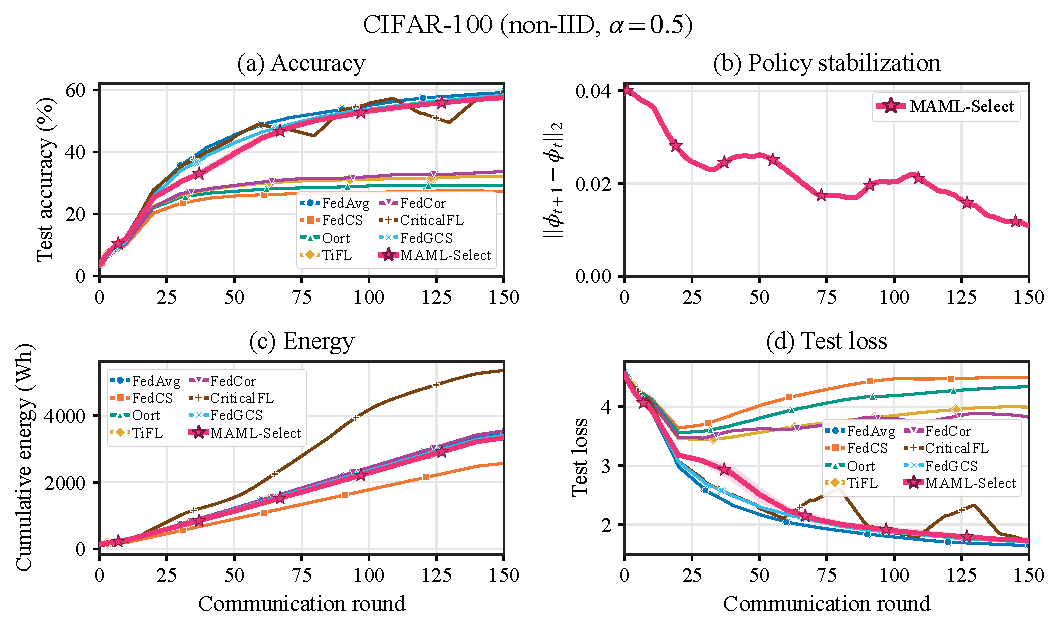
\includegraphics[width=0.94\columnwidth]{fig_convergence_boxed.pdf}
\caption{\revision{CIFAR-100 convergence over 150 rounds. The panels report (a)~accuracy, (b)~the selector meta-update magnitude $\lVert\phi_{t+1}-\phi_t\rVert_2$ for MAML-Select \revtwo{, which shrinks and then settles at a small non-zero level, the behaviour Corollary~\ref{cor:rate} predicts under a drifting query objective}, (c)~cumulative modelled energy consumption, and (d)~test loss.}}
\label{fig:convergence}
\end{figure}

\revision{Fig.~\ref{fig:effscale}(a) shows the efficiency and accuracy trade-off. Relative to FedAvg over shared seeds, MAML-Select lowers cumulative TFLOPs by $12.9\%$, $21.5\%$ and $1.7\%$ and modelled energy by $16.4\%$, $24.8\%$ and $4.7\%$ on the three datasets, for accuracy changes of $-0.1$, $-3.8$ and $-1.5$ percentage points, so the gain is resource efficiency at competitive accuracy.}

\begin{figure}[!tb]
\centering
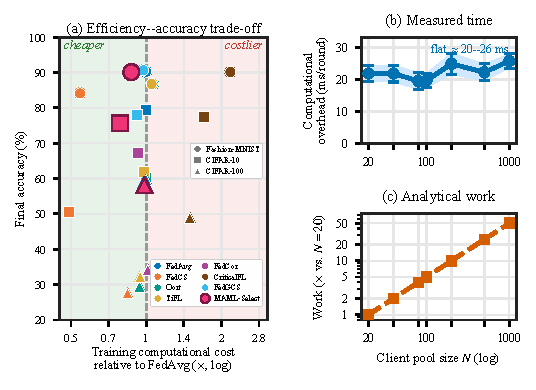
\includegraphics[width=0.94\columnwidth]{fig_efficiency_scaling_boxed.pdf}
\caption{\revision{(a)~Efficiency and accuracy trade-off, where the $x$-axis is cumulative training cost relative to FedAvg on a log scale and $x<1$ is cheaper, the $y$-axis is final accuracy, and marker shape encodes the dataset. (b)~Measured per-round selection overhead, as a mean with $95\%$ confidence intervals over $10$ rounds. (c)~The operation count $C(N,K)$ of~\eqref{eq:selector_complexity} with $P=4{,}673$, normalized to $N=20$, both varying $N$ at a $10\%$ selection rate.}}
\label{fig:effscale}
\end{figure}

\revision{Fairness uses Jain's index on the selection counts $\{p_i\}_{i=1}^{N}$, $J=\big(\sum_{i} p_i\big)^2 / \big(N\sum_{i} p_i^2\big)$, which lies in $[1/N,1]$ and equals $1$ for even selection. Coverage $\mathrm{Cov}=\tfrac{100}{N}\,|\{\,i:\sum_{t} a_{i,t}\ge 1\,\}|$ is the percentage selected at least once. MAML-Select reaches $100\%$ coverage on every dataset, with a Jain index of $0.61$ to $0.78$.} \revtwo{The two differ. Coverage is guaranteed by the exploration slot (Proposition~\ref{prop:coverage}) whatever the learned ranking, whereas the Jain index measures how evenly the remaining $K-\varepsilon$ places are spread, and Sec.~\ref{sec:tier} shows the lower index reflects a preference for fast devices.}

\subsection{\revtwo{Tier-Level Participation}}\label{sec:tier}
\revtwo{Coverage says how evenly clients are used but not which ones, so we also measured the share of selections per device tier on CIFAR-100 against a pool composition of $0.20/0.50/0.30$. FedCS collapses onto the fast tier, placing all of its selections in Tier~3 and reaching only $10\%$ coverage. FedAvg tracks the pool at $0.196/0.495/0.309$ and FedGCS at $0.217/0.472/0.311$, both with full coverage. MAML-Select shifts toward the fast tier at $0.116/0.446/0.437$, yet keeps the slow tier represented at full coverage. What matters is the distinction between preferring fast devices and excluding slow ones, and only the former is compatible with Proposition~\ref{prop:coverage}.}

\subsection{\revtwo{Coverage Without the Forced Cold Start}}\label{sec:fairness_recheck}
\revtwo{The cold start visits every client once in the first $10$ of $200$ rounds, so the coverage figures could be an artifact of that schedule. Recomputing both metrics over the policy-driven rounds alone, across all $74$ distinct MAML-Select runs and every $\lambda$, inner-step, width and feature-ablation setting, coverage is $100\%$ in every individual run. Pooled over those runs Jain's index falls only slightly, from $0.755$ to $0.737$, $0.411$ to $0.367$, and $0.802$ to $0.785$. Pooling averages over settings, including large $\lambda$, so these sit below the default values of Table~\ref{tab:main_summary}.}

\begin{proposition}[\revtwo{Coverage from the exploration slot alone}]\label{prop:coverage}
\revtwo{Suppose every client is available each round and $\varepsilon\ge 1$. Then, after the cold start, every client is selected at least once in any window of $N-1$ consecutive rounds, whatever the policy $h_\phi$.}
\end{proposition}
\begin{proof}
\revtwo{Staleness obeys $\tau_{i,t+1}=0$ if $i\in\mathcal{S}_t$ and $\tau_{i,t+1}=\tau_{i,t}+1$ otherwise, and the slot goes to a client of maximal staleness. Fix $j$ and a window starting at $t$, and suppose $j$ is never selected in it. For $j$ to miss the slot at round $s\ge t$, some $i_s\neq j$ with $\tau_{i_s,s}\ge\tau_{j,s}$ takes it and resets to $0$. Since $i_s$ resets at $s$, its staleness at $s'>s$ is $s'-s-1$, so blocking $j$ again would need $s'-s-1\ge\tau_{j,t}+(s'-t)$, that is $t-s\ge\tau_{j,t}+1\ge 1$, which is impossible for $s\ge t$. Each of the other $N-1$ clients blocks $j$ at most once, so $j$ is selected within $N-1$ rounds. Selection through the learned ranking also resets $\tau_j$, which can only shorten the window.}
\end{proof}
\revtwo{With $N=100$ and $T=200$ the condition is met twice over, so coverage holds in every run. The cold start seeds the feedback buffer but does not create the result, and Jain's index depends mildly on it, so we report both.}

\subsection{\revtwo{Selector Convergence and Objective Drift}}\label{sec:selector_convergence}
\revtwo{We instrument a full $199$-round run on each dataset, recording the inner-step change, the realized query objective, and the meta-update magnitude. Lemma~\ref{stmt:inner} is confirmed exactly, since the inner step is non-increasing on the support loss in $198$ of $198$ adapted rounds on all three datasets, so $\beta=10^{-2}$ lies inside the admissible range in practice.}

\revtwo{The query objective is not monotone on any dataset. On Fashion-MNIST it falls from $3.312$ to $0.015$ with round-to-round jumps as large as $2.672$, on CIFAR-10 it moves within $[0.015,1.023]$ with jumps to $0.703$, and on CIFAR-100 within $[0.055,3.704]$ with jumps to $3.612$. A fixed objective descended with $\eta\le 1/L_q$ cannot produce increases of this size, so the sequence is direct evidence that $q_t$ changes between rounds, which is the drift term $V_T$ of Corollary~\ref{cor:rate}. Logging both objectives at a common iterate measures it directly. Over $198$ rounds it is $-2.89$ on Fashion-MNIST, $0.51$ on CIFAR-10, and $1.79$ on CIFAR-100, so $\lvert V_T\rvert/T$ is at most $0.015$. The partial sums flatten instead of growing with the horizon, which places all three runs in the $V_T=o(T)$ regime of Remark~\ref{rem:reading}, and Fashion-MNIST is negative and so falls in the benign case that remark identifies. These are single instrumented runs, so they measure the drift term without characterizing its distribution.}

\subsection{\revision{Sensitivity and Ablation}}
\revision{We probe the cost trade-off $\lambda$, the inner-loop steps, the selector width, and the six-feature state, each on the dataset where it is most informative. Fig.~\ref{fig:lambda_sensitivity} reports the $\lambda$ sweep. A larger $\lambda$ weights cheaper clients more, so cost and energy fall on both datasets. Accuracy stays within about one point on Fashion-MNIST, whereas on CIFAR-10 the trade-off is sharper, falling from $64.9\%$ at $\lambda=0.1$ to $56.3\%$ at $\lambda=5$ while cost drops by about $26\%$ and energy by about $30\%$. Fairness also falls at large $\lambda$, so we keep $\lambda=0.5$.}

\begin{figure}[!tb]
\centering
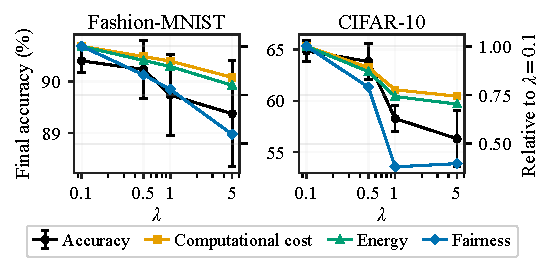
\includegraphics[width=0.94\columnwidth]{fig_lambda_two_dataset_boxed.pdf}
\caption{\revision{Sensitivity to the cost trade-off $\lambda$ on Fashion-MNIST (left) and CIFAR-10 (right). The black curve is accuracy, and cost, energy and fairness are normalized to their $\lambda=0.1$ values.} \revtwo{The CIFAR-10 sweep uses the $100$-round protocol of Table~\ref{tab:design_ablation}.}}
\label{fig:lambda_sensitivity}
\end{figure}

\revision{Table~\ref{tab:design_ablation} depicts the choices of two ablations. On CIFAR-10, a single inner step gives the highest accuracy ($63.8\%$ at $100$ rounds) and the lowest overhead ($38.7$ versus $45.2$~ms at five steps), so we use one step. On Fashion-MNIST, accuracy stays within about $0.6$ points as $h$ grows over $\{16,32,64,128\}$, or $401$ to $17{,}537$ weights, so $h=64$ is robust.}

\begin{table}[!t]
\centering
\color{black}
\caption{\revtwo{Design ablations, grouped by the choice being varied. Accuracy is the mean $\pm$ standard deviation over three seeds. Cost is selection overhead in milliseconds for the first two groups and cumulative TFLOPs for the third, and a blank marks a quantity not recorded. The CIFAR-10 group runs for $100$ rounds rather than the $200$ of Table~\ref{tab:main_summary}, so its accuracies are read within the group. Defaults are in bold.}}
\label{tab:design_ablation}
\footnotesize
\setlength{\tabcolsep}{4pt}
\renewcommand{\arraystretch}{1.08}
\begin{tabular*}{\columnwidth}{@{\extracolsep{\fill}}lrrr@{}}
\toprule
\revision{Setting} & \revision{Acc.\ (\%)} & \revision{Cost} & \revision{Jain} \\
\midrule
\multicolumn{4}{@{}l}{\revision{\textit{Inner-loop steps, CIFAR-10, cost in ms}}} \\
\revision{\textbf{1}} & \revision{\textbf{63.8$\pm$1.8}} & \revision{\textbf{38.7}} & \\
\revision{2} & \revision{63.1$\pm$1.8} & \revision{39.8} & \\
\revision{5} & \revision{62.2$\pm$2.4} & \revision{45.2} & \\
\addlinespace[2pt]
\multicolumn{4}{@{}l}{\revision{\textit{Selector width $h$, Fashion-MNIST, cost in ms}}} \\
\revision{16} & \revision{90.0$\pm$0.3} & \revision{10.2} & \\
\revision{32} & \revision{90.6$\pm$0.3} & \revision{10.4} & \\
\revision{\textbf{64}} & \revision{\textbf{90.1$\pm$0.5}} & \revision{\textbf{10.2}} & \\
\revision{128} & \revision{90.3$\pm$0.7} & \revision{11.6} & \\
\addlinespace[2pt]
\multicolumn{4}{@{}l}{\textit{State features, Fashion-MNIST, $200$ rounds, cost in TFLOPs}} \\
\textbf{Full state vector} & \textbf{90.23$\pm$0.55} & \textbf{122} & \textbf{0.78} \\
w/o loss & 90.16$\pm$0.66 & 123 & 0.79 \\
w/o gradient norm & 90.30$\pm$0.24 & 122 & 0.78 \\
w/o latency & 90.14$\pm$0.14 & 119 & 0.70 \\
w/o battery & 89.90$\pm$0.44 & 122 & 0.79 \\
w/o frequency & 90.47$\pm$0.13 & 115 & 0.65 \\
w/o staleness & 90.37$\pm$0.19 & 123 & 0.78 \\
\bottomrule
\end{tabular*}
\end{table}

\revision{The last group of Table~\ref{tab:design_ablation} removes one state feature at a time. Accuracy changes stay within about $0.35$ points, so the policy is robust to any single removal. The largest drop comes from the battery feature ($-0.33$~pp), with latency and loss also contributing. Removing the frequency feature raises accuracy slightly but lowers the Jain index the most, from $0.78$ to $0.65$, so the participation features chiefly protect fairness.}

\subsection{\revtwo{Behaviour Under Severe Heterogeneity}}\label{sec:alpha01}
\revtwo{The results above use a Dirichlet concentration of $\alpha=0.5$. Repeating the comparison at $\alpha=0.1$ over three seeds, under the protocol of Section~\ref{sec:results_acc} in all other respects, gives MAML-Select $55.8\pm6.3$ TFLOPs against $140.0\pm1.3$ for FedAvg on Fashion-MNIST and $4423\pm581$ against $8342\pm89$ on CIFAR-10. These are reductions of $60\%$ and $47\%$, at $p=0.002$ and $p=0.007$ on a paired test. Accuracy falls, to $83.4\pm4.3$ against $86.6\pm2.7$ on Fashion-MNIST and $41.2\pm6.2$ against $58.6\pm7.7$ on CIFAR-10, with FedGCS between the two at $85.1\pm2.2$ and $50.5\pm16.9$. The cost term of~\eqref{eq:cost} concentrates selection on fast devices, and at $\alpha=0.1$ those devices hold a narrower slice of the label space, so the cohort sees fewer classes per round. This is the operating boundary of the method. MAML-Select suits moderate heterogeneity, and at $\alpha=0.1$ the compute saving carries an accuracy cost on CIFAR-10.}

% =====================================================================
% VI. CONCLUSION
% =====================================================================
\FloatBarrier
\section{Conclusion and Future Work}
\revision{We introduced MAML-Select, an online adaptive client-selection framework for heterogeneous FL that learns a lightweight ranking policy over learning feedback and system state, and adapts it before each selection decision.
Across Fashion-MNIST, CIFAR-10, and CIFAR-100 it holds competitive accuracy while lowering cumulative computational cost, modelled energy, and round latency. The $\lambda$ study shows a mild trade-off on Fashion-MNIST and a sharper one on CIFAR-10, and the ablations confirm that a single inner step, a compact policy network, and the full six-feature state suffice.} \revtwo{The evaluation covers two heterogeneity levels, one cohort size and three vision datasets, and a no-adaptation control is left open. Section~\ref{sec:alpha01} marks the boundary at $\alpha=0.1$.} \revision{Future work will broaden the evaluation across pool sizes and naturally federated benchmarks, and will study an asynchronous extension together with a differentially private client-state vector so that selection does not leak device information.}

\balance
%=====================================================================
% REFERENCES
% =====================================================================
\vspace{-1mm}
% Tighten inter-reference spacing to keep the bibliography compact.
\let\OLDthebibliography\thebibliography
\renewcommand\thebibliography[1]{%
  \OLDthebibliography{#1}%
  \setlength{\itemsep}{0pt plus 0.2pt}%
  \setlength{\parsep}{0pt}%
  \setlength{\topsep}{0pt}}
{\scriptsize
\begin{thebibliography}{10}
\providecommand{\url}[1]{#1}
\csname url@samestyle\endcsname
\providecommand{\newblock}{\relax}
\providecommand{\bibinfo}[2]{#2}
\providecommand{\BIBentrySTDinterwordspacing}{\spaceskip=0pt\relax}
\providecommand{\BIBentryALTinterwordstretchfactor}{4}
\providecommand{\BIBentryALTinterwordspacing}{\spaceskip=\fontdimen2\font plus
\BIBentryALTinterwordstretchfactor\fontdimen3\font minus \fontdimen4\font\relax}
\providecommand{\BIBforeignlanguage}[2]{{%
\expandafter\ifx\csname l@#1\endcsname\relax
\typeout{** WARNING: IEEEtran.bst: No hyphenation pattern has been}%
\typeout{** loaded for the language `#1'. Using the pattern for}%
\typeout{** the default language instead.}%
\else
\language=\csname l@#1\endcsname
\fi
#2}}
\providecommand{\BIBdecl}{\relax}
\BIBdecl

\bibitem{mcmahan2017communication}
B.~McMahan \emph{et al.}, ``Communication-efficient learning of deep networks from decentralized data,'' in \emph{Proc. AISTATS}.\hskip 1em plus 0.5em minus 0.4em\relax PMLR, 2017, pp. 1273--1282.

\bibitem{karimireddy2020scaffold}
S.~P. Karimireddy \emph{et al.}, ``{SCAFFOLD}: Stochastic controlled averaging for federated learning,'' in \emph{Proc. ICML}.\hskip 1em plus 0.5em minus 0.4em\relax PMLR, 2020, pp. 5132--5143.

\bibitem{mai2024study}
V.~S. Mai, R.~J. La, and T.~Zhang, ``A study of enhancing federated learning on non-{IID} data with server learning,'' \emph{IEEE Transactions on Artificial Intelligence}, vol.~5, no.~11, pp. 5589--5604, 2024.

\bibitem{tapwal2026stragglers}
\revision{R.~Tapwal, ``Stragglers reimagined: Explainability-driven adaptive federated learning for resource constrained {IoMT} system,'' \emph{IEEE Transactions on Artificial Intelligence}, vol.~7, no.~2, pp. 1002--1011, 2026.}

\bibitem{forootani2026asynchronous}
\revision{A.~Forootani and R.~Iervolino, ``Asynchronous federated learning with nonconvex client objective functions and heterogeneous dataset,'' \emph{IEEE Transactions on Artificial Intelligence}, vol.~7, no.~5, pp. 2610--2624, 2026.}

\bibitem{borazjani2026redefining}
\revision{K.~Borazjani \emph{et al.}, ``Redefining non-{IID} data in federated learning for computer vision tasks,'' \emph{IEEE Transactions on Artificial Intelligence}, 2026, early access.}

\bibitem{nishio2019client}
T.~Nishio and R.~Yonetani, ``Client selection for federated learning with heterogeneous resources in mobile edge,'' in \emph{Proc. IEEE ICC}.\hskip 1em plus 0.5em minus 0.4em\relax IEEE, 2019, pp. 1--7.

\bibitem{chai2020tifl}
Z.~Chai \emph{et al.}, ``{TiFL}: A tier-based federated learning system,'' in \emph{Proc. ACM HPDC}, 2020, pp. 125--136.

\bibitem{lai2021oort}
F.~Lai, X.~Zhu, H.~V. Madhyastha, and M.~Chowdhury, ``{Oort}: Efficient federated learning via guided participant selection,'' in \emph{Proc. USENIX OSDI}, 2021, pp. 19--35.

\bibitem{tang2022fedcor}
M.~Tang \emph{et al.}, ``{FedCor}: Correlation-based active client selection strategy for heterogeneous federated learning,'' in \emph{Proc. IEEE/CVF CVPR}.\hskip 1em plus 0.5em minus 0.4em\relax IEEE, 2022, pp. 10\,102--10\,111.

\bibitem{xu2024federated}
Y.~Xu \emph{et al.}, ``Federated learning with client selection and gradient compression in heterogeneous edge systems,'' \emph{IEEE Transactions on Mobile Computing}, vol.~23, no.~5, pp. 5446--5461, 2024.

\bibitem{yan2023criticalfl}
G.~Yan, H.~Wang, X.~Yuan, and J.~Li, ``{CriticalFL}: A critical learning periods augmented client selection framework for efficient federated learning,'' in \emph{Proc. ACM SIGKDD}, 2023, pp. 5034--5044.

\bibitem{ning2024fedgcs}
Z.~Ning \emph{et al.}, ``{FedGCS}: A generative framework for efficient client selection in federated learning via gradient-based optimization,'' in \emph{Proceedings of the 33rd International Joint Conference on Artificial Intelligence}, 2024, pp. 4760--4768.

\bibitem{wang2020optimizing}
H.~Wang, Z.~Kaplan, D.~Niu, and B.~Li, ``Optimizing federated learning on non-{IID} data with reinforcement learning,'' in \emph{IEEE INFOCOM}.\hskip 1em plus 0.5em minus 0.4em\relax IEEE, 2020, pp. 1698--1707.

\bibitem{pan2024contextual}
Q.~Pan, H.~Cao, Y.~Zhu, J.~Liu, and B.~Li, ``Contextual client selection for efficient federated learning over edge devices,'' \emph{IEEE Transactions on Mobile Computing}, vol.~23, no.~6, pp. 6538--6548, 2024.

\bibitem{kazemi2026robust}
\revision{K.~Kazemi, M.~H. Badiei, and H.~Kebriaei, ``Robust peer-to-peer federated learning with deep reinforcement learning based client selection against data poisoning attacks,'' \emph{IEEE Transactions on Artificial Intelligence}, vol.~7, no.~1, pp. 262--271, 2026.}

\bibitem{finn2017model}
C.~Finn, P.~Abbeel, and S.~Levine, ``Model-agnostic meta-learning for fast adaptation of deep networks,'' in \emph{Proc. ICML}.\hskip 1em plus 0.5em minus 0.4em\relax PMLR, 2017, pp. 1126--1135.

\bibitem{fallah2020personalized}
A.~Fallah, A.~Mokhtari, and A.~Ozdaglar, ``Personalized federated learning with theoretical guarantees: A model-agnostic meta-learning approach,'' \emph{Proc. NeurIPS}, vol.~33, pp. 3557--3568, 2020.

\bibitem{tran2026fedimp}
\revision{H.~A. Tran, C.~Ta, and T.~X. Tran, ``{FedImp}: Enhancing federated learning convergence with impurity-based weighting,'' \emph{IEEE Transactions on Artificial Intelligence}, vol.~7, no.~3, pp. 1652--1665, 2026.}

\bibitem{arisdakessian2026vox}
\revision{S.~Arisdakessian, O.~A. Wahab, A.~Mourad, and H.~Otrok, ``Towards vox populi in federated learning: A fair and inclusive client selection framework,'' \emph{IEEE Transactions on Artificial Intelligence}, vol.~7, pp. 1997--2011, 2026.}

\bibitem{wu2018light}
X.~Wu, R.~He, Z.~Sun, and T.~Tan, ``A light {CNN} for deep face representation with noisy labels,'' \emph{IEEE Transactions on Information Forensics and Security}, vol.~13, no.~11, pp. 2884--2896, 2018.

\bibitem{he2016deep}
K.~He, X.~Zhang, S.~Ren, and J.~Sun, ``Deep residual learning for image recognition,'' in \emph{Proc. IEEE CVPR}.\hskip 1em plus 0.5em minus 0.4em\relax IEEE, 2016, pp. 770--778.

\bibitem{li2020federated}
T.~Li, A.~K. Sahu, A.~Talwalkar, and V.~Smith, ``Federated learning: Challenges, methods, and future directions,'' \emph{IEEE Signal Processing Magazine}, vol.~37, no.~3, pp. 50--60, 2020.


\end{thebibliography}
}

\end{document}
